\section{Interlinking the chain}
In order to be able to utilize the superblocks for constructing succinct proofs of PoW it is proposed that block headers additionally include the \emph{interlink} data structure. The interlink of a block $b$ contains pointers to the most recent $\mu-$level ancestor of $b$ for every $\mu \leq log(\chain)$. The interlink turns the blockchain into a skiplist-like data structure, as illustrated in Figure~\ref{fig:hierarchical_ledger}.

\begin{figure}[h!]
	\begin{center}
		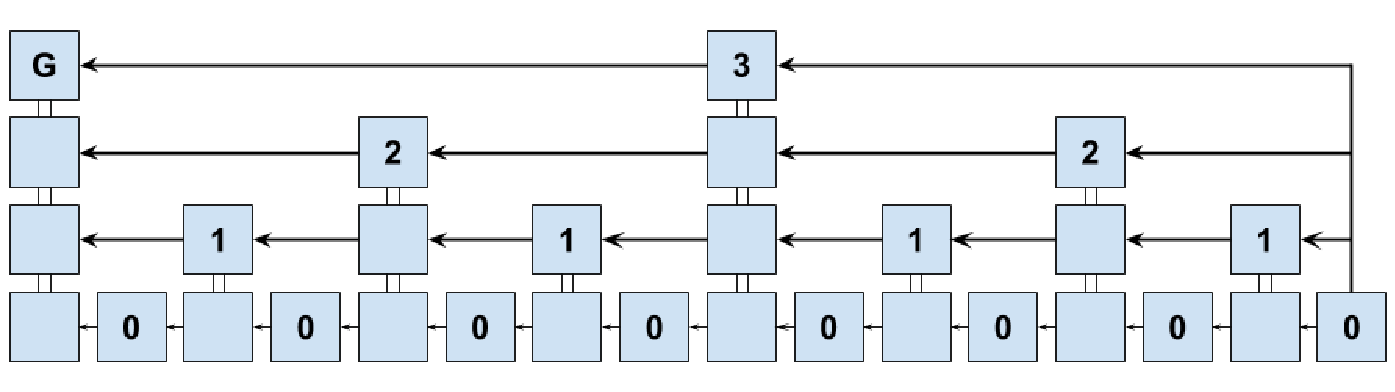
\includegraphics[width=0.8\columnwidth]{figures/hierarchical-ledger.pdf}
	\end{center}
	\caption{The hierarchical blockchain. Each block has a pointer to its nearest $\mu-$level ancestor.}
	\label{fig:hierarchical_ledger}
\end{figure}

Updated interlink information has to be included in each block during mining. The algorithm for the honest miner is given in Algorithm~\ref{alg:update_interlink_soft_fork} as described in~\cite{popow}. The updateInterlink algorithm accepts a block $B'$, which already contains an interlink strucure, and evaluates the interlink that has to be included as part of the next block. It copies the existing interlink and then modifies its pointers from level 0 to $level(B')$, so that they point to block $B'$. For every freshly mined block relayed to the network, a node has now additionally to check the validity of the interlink data included. 

\begin{algorithm}[h]
		\caption{\label{alg:update_interlink_soft_fork}updateInterlink~\cite{popow}}
		\begin{algorithmic}[1]
				\Function{\sf updateInterlinkVelvet}{$B'$}
						\Let{\textsf{interlink}}{B'.\textsf{interlink}}
						\For{$\mu = 0$ to $\textsf{level}(B')$}
								\Let{\textsf{interlink}[\mu]}{\textsf{id}(B')}
						\EndFor
						\State\Return$\textsf{interlink}$
				\EndFunction
		\end{algorithmic}
\end{algorithm}

For the rest of this work, we use the notation defined in the superblock NIPoPows paper~\cite{nipopows}, which we rewrite here so as to serve as an easier point of reference.
Blockchains are sequences but it is more convenient to use set notation for some operations. Specifically $B \in \chain$, $\chain_1 \subseteq \chain_2$ and $\emptyset$ have the obvious meaning. $\chain_1 \cup \chain_2$ is the chain obtained by sorting the blocks contained in both $\chain_1$ and $\chain_2$ into a sequence (this may be not always defined). We will freely use set builder notation $\{ B \in \chain: p(B)\}$. $\chain_1 \cap \chain_2$ is the chain $\{B: B \in \chain_1 \wedge B \in \chain_2 \}$. The lowest common ancestor is $LCA(\chain_1, \chain_2) = (\chain_1 \cap \chain_2)[-1]$. if $\chain_1[0] = \chain_2[0]$ and $\chain_1[-1] = \chain_2[-1]$, we say that chains $\chain_1, \chain_2$ \emph{span} the same block range. 

It is frequently useful to construct a chain containing only the superblocks of another chain. Given $\chain$ and level $\mu$, the \emph{upchain} $\chain\upchain$ is defined a $\{B \in \chain: level(B) \geq \mu \}$. A chain containing only $\mu-$superblocks is calles a $\mu-$superchain. It is also useful, given a $\mu-$superchain to go back to the regular chain $\chain$. Given chains $\chain' \subset \chain$, the \emph{downchain} $\chain' \downchain_\chain$ is defined as $\{ \chain[\chain'[0]:\chain'[-1]] \}$. $\chain$ is the \emph{underlying chain} of $\chain'$. The underlying chain is often implied by context, so we will simply write $\chain' \downchain$. By the above definition, the $\chain' \uparrow$ is absolute: $\left( \chain \uparrow^\mu \right)^{\mu + i} = \chain \uparrow^{\mu + i}$. Given a set of consecutive rounds $S = \{ r, r+1, \cdots, r+j \} \subseteq \mathbb{N}$, we define $\chain^S = \{ B \in \chain: B \text{ was generated during S} \}$.